\chapter{Benchmarks}
\label{benchmarks}

This appendix gives the source code of the benchmark programs used to
evaluate the distributed performance of PrologPF.  Graphical representations
of the search trees are included for each benchmark.

%%%%%%%%%%%%%%%%%%
\section{Queens} %
%%%%%%%%%%%%%%%%%%
\label{queens_benchmark}

The Queens benchmark places $N$ queens on an $N$ by $N$ chessboard, such that
no pair of queens are on the same horizontal, vertical or diagonal.

\begin{figure}[htb]
\vspace{5mm} \hbox to \hsize{\hfill \psfig{file={benchmarks/ps/q8_tree.ps}} \hfill}
\caption{8 Queens: search tree.}
\vspace{5mm}
\end{figure}

\begin{figure}[htb]
\vspace{5mm} \hbox to \hsize{\hfill \psfig{file={benchmarks/ps/q10_tree.ps}} \hfill}
\caption{10 Queens: search tree.}
\vspace{5mm}
\label{q10_tree}
\end{figure}

\begin{verbatim}
:- main([f_utils,o_kutils]).

% get_solutions(N,S) succeeds if S is a solution for
%  the placement of N queens on an NxN chessboard.

get_solutions(Board_size, Soln) :- solve(Board_size, [], Soln). 

% solve(N, Initial, Final) succeeds if Final is a solution
%  to the NxN queens problem and Final is an extension of
%  the partial solution in Initial.

solve(Bs, [square(Bs, Y) | L], [square(Bs, Y) | L]).
solve(Board_size, Initial, Final) :-
    newsquare(Initial, Next, Board_size),
    solve(Board_size, [Next | Initial], Final).
\end{verbatim}      % manual final formatting
\pagebreak          % manual final formatting
\begin{verbatim}
% newsquare(Initial, Square, N) acts as a generator for
%  'safe' squares in the next column to those already
%  allocated in the partial solution in Initial.

newsquare([square(I,J) | Rest], square(X, Y), Boardsize) :-
    I < Boardsize, X is I + 1, snint(Y, Boardsize),
    notthreatened(I, J, X, Y), safe(X, Y, Rest).
newsquare([], square(1, X), Boardsize) :- snint(X, Boardsize).

% snint(X,N) acts as generator for X = N down to 1.

snint(X, X).
snint(N, NPlusOneOrMore) :- M is NPlusOneOrMore - 1, M > 0,
    snint(N,M).

% notthreatened(I,J,X,Y) succeeds if a queen on square (I,J)
%  does not attack square (X,Y).

notthreatened(I, J, X, Y) :- I \== X, J \== Y, 
    U1 is I - J, V1 is X - Y, U1 \== V1,
    U2 is I + J, V2 is X + Y, U2 \== V2, !.

\end{verbatim}      % manual final formatting
\pagebreak          % manual final formatting
\begin{verbatim}
% safe(X,Y,Initial) succeeds if square (X,Y) is not attacked
%  by any queens in the partial solution Initial.

safe(X, Y, []) :- !.
safe(X, Y, [square(I, J) | L]) :-
    notthreatened(I, J, X, Y), safe(X, Y, L).

% o_query is called by the PrologPF system to obtain the
%  solutions.

o_query :- get_solutions(8,X), o_ksoln(X).  % or 10 for 10-queens

% o_kloop is a top-level system predicate which responds to
%  the commands from the control processor.

:- o_kloop.
\end{verbatim}

%%%%%%%%%%%%%%%%%%%%%%%
\section{Pentominoes} %
%%%%%%%%%%%%%%%%%%%%%%%
\label{pent_benchmark}
%\enlargethispage{\baselineskip}  % manual final formatting

The Pentominoes benchmark places twelve geometric shapes on a twenty by three board.

\begin{figure}[htb]
\vspace{5mm} \hbox to \hsize{\hfill \psfig{file={benchmarks/ps/pent_tree.ps}} \hfill}
\caption{Pentominoes: search tree.}
\vspace{5mm}
\label{pent_tree}
\end{figure}

\begin{verbatim}
:- main([f_utils,o_kutils]).

% solution(H) succeeds if H is a solution to the problem.

solution(H) :- initial_state(Si),
               can_reach(Si,Sf),
               final_state(Sf),
               Sf = state(_,_,H).

% initial_state(S) builds the term S representing the initial
%  state of the problem, using gen_board to build each
%  column of the 20x3 board.

initial_state(state(Board,[1,2,3,4,5,6,7,8,9,10,11,12],[])) :-
    gen_board(20,Board), !.

gen_board(0,[]) :- !.
gen_board(N,[no_piece,no_piece,no_piece,border|T]) :-
    N > 0,
    I is (N - 1),
    gen_board(I,T).
\end{verbatim}      % manual final formatting
\pagebreak          % manual final formatting
\begin{verbatim}
% final_state(S) succeeds if S indicates all pieces have been
%  placed.

final_state(state(_,[],_)) :- !.

% can_reach(S1,S2) succeeds if the second state of play
%  represented by S2 can be reached from state S1.

can_reach(S1,S2) :- trans(S1,S), S = S2.
can_reach(S1,S2) :- trans(S1,S), can_reach(S,S2).

% trans(S1,S2) succeeds if state S2 can be reached from 
%  state S1 through the valid placement of one of the
%  remaining pieces.

trans(State,New_State) :-
    State = state(Board,Pieces,History),
    del(Piece,Pieces,New_Pieces),
    pent(Piece,Orientation,Pattern),
    play_pent(Board,Pattern,New_Board),
    New_State = state(New_Board,New_Pieces,
                      [[Piece,Orientation] | History]).

% del(X,L1,L2) succeeds if list L2 is equal to list
%  L1 with the removal of an element equal to X.  It
%  is used as a generator for elements of L1 (pieces).

del(X,[X|Y],Y).
del(X,[Y|Z], [Y|Z1]) :- del(X,Z,Z1).

% play_pent fits the pattern represented by a pentomino
%  of a given orientation onto the board, and generates
%  the remaining new board.

play_pent(Board,Pattern,New_Board) :-
    match(Board,Pattern,Board1),
    trim(Board1,New_Board), !.

% trim(B1, B2) succeeds if board B2 is the pattern
%  representing the remaining clear squares on the
%  board excluding the pieces and border of the board B1.

trim([],[]) :- !.
trim([border|T],Board) :- trim(T,Board).
trim([piece|T],Board) :- trim(T,Board).
trim(Board,Board) :- Board = [no_piece|_].

% match succeeds of the pattern representing a selected
%  piece can be placed on the board.

match(Board,[],Board) :- !.
match([piece|Tb],[dnm|Tp],[piece|Tnb]) :-
    match(Tb,Tp,Tnb).
match([piece|Tb],[op|Tp],[piece|Tnb]) :-
    match(Tb,Tp,Tnb).
match([no_piece|Tb],[np|Tp],[piece|Tnb]) :-
    match(Tb,Tp,Tnb).
match([no_piece|Tb],[dnm|Tp],[no_piece|Tnb]) :-
    match(Tb,Tp,Tnb).
match([border|Tb],[dnm|Tp],[border|Tnb]) :-
    match(Tb,Tp,Tnb).


% the following terms represent the patterns of all 12
%  pentominoes in each orientation.

pent(1,1,[np,np,np,dnm,np,dnm,np]).
pent(1,2,[np,op,np,dnm,np,np,np]).
pent(1,3,[np,np,dnm,dnm,np,dnm,dnm,dnm,np,np]).
pent(1,4,[np,np,dnm,dnm,dnm,np,dnm,dnm,np,np]).

pent(2,1,[np,op,dnm,np,np,np,dnm,dnm,np]).

pent(3,1,[np,np,np,dnm,dnm,dnm,np,dnm,dnm,dnm,np]).
pent(3,2,[np,np,np,dnm,np,dnm,dnm,dnm,np]).
pent(3,3,[np,dnm,op,op,np,dnm,np,np,np]).
pent(3,4,[np,op,op,dnm,np,op,op,dnm,np,np,np]).

pent(4,1,[np,op,dnm,op,np,op,dnm,np,np,np]).
pent(4,2,[np,op,op,dnm,np,np,np,dnm,np]).
pent(4,3,[np,dnm,np,np,np,dnm,dnm,dnm,np]).
pent(4,4,[np,np,np,dnm,dnm,np,dnm,dnm,dnm,np]).

pent(5,1,[np,np,dnm,np,np,np]).
pent(5,2,[np,np,dnm,dnm,np,np,dnm,dnm,np]).
pent(5,3,[np,np,op,dnm,np,np,np]).
pent(5,4,[np,np,dnm,dnm,np,np,dnm,dnm,dnm,np]).
pent(5,5,[np,np,np,dnm,np,np]).
pent(5,6,[np,np,np,dnm,dnm,np,np]).
pent(5,7,[np,dnm,dnm,dnm,np,np,dnm,dnm,np,np]).
pent(5,8,[np,dnm,dnm,np,np,dnm,dnm,np,np]).

pent(6,1,[np,dnm,op,np,np,dnm,np,np]).
pent(6,2,[np,op,op,dnm,np,np,op,dnm,dnm,np,np]).
pent(6,3,[np,np,op,dnm,dnm,np,np,dnm,dnm,dnm,np]).
pent(6,4,[np,np,dnm,np,np,dnm,dnm,np]).

pent(7,1,[np,dnm,dnm,dnm,np,dnm,dnm,dnm,np,dnm,dnm,np,np]).
pent(7,2,[np,dnm,dnm,dnm,np,dnm,dnm,dnm,np,dnm,dnm,dnm,np,np]).
pent(7,3,[np,np,dnm,dnm,np,dnm,dnm,dnm,np,dnm,dnm,dnm,np]).
pent(7,4,[np,np,dnm,dnm,dnm,np,dnm,dnm,dnm,np,dnm,dnm,dnm,np]).

pent(8,1,[np,dnm,dnm,dnm,np,dnm,dnm,dnm,np,np,dnm,dnm,np]).
pent(8,2,[np,dnm,dnm,dnm,np,np,dnm,dnm,np,dnm,dnm,dnm,np]).
pent(8,3,[np,dnm,dnm,dnm,np,dnm,dnm,np,np,dnm,dnm,dnm,np]).
pent(8,4,[np,dnm,dnm,np,np,dnm,dnm,dnm,np,dnm,dnm,dnm,np]).

pent(9,1,[np,np,op,dnm,dnm,np,np,dnm,dnm,np]).
pent(9,2,[np,dnm,np,np,np,dnm,dnm,np]).
pent(9,3,[np,op,op,dnm,np,np,np,dnm,dnm,np]).
pent(9,4,[np,np,dnm,np,np,dnm,dnm,dnm,np]).
pent(9,5,[np,op,dnm,np,np,op,dnm,dnm,np,np]).
pent(9,6,[np,op,dnm,op,np,np,dnm,np,np]).
pent(9,7,[np,op,dnm,np,np,np,dnm,dnm,dnm,np]).
pent(9,8,[np,op,dnm,np,np,np,dnm,np]).

pent(10,1,[np,np,dnm,op,np,dnm,dnm,np,np]).
pent(10,2,[np,np,op,dnm,dnm,np,op,dnm,dnm,np,np]).
pent(10,3,[np,op,op,dnm,np,np,np,dnm,dnm,dnm,np]).
pent(10,4,[np,dnm,np,np,np,dnm,np]).

pent(11,1,[np,dnm,dnm,dnm,np,dnm,dnm,np,np,dnm,dnm,np]).
pent(11,2,[np,dnm,dnm,dnm,np,dnm,dnm,dnm,np,np,dnm,dnm,dnm,np]).
pent(11,3,[np,dnm,dnm,dnm,np,np,dnm,dnm,dnm,np,dnm,dnm,dnm,np]).
pent(11,4,[np,dnm,dnm,np,np,dnm,dnm,np,dnm,dnm,dnm,np]).

pent(12,1,[np,dnm,dnm,dnm,np,dnm,dnm,dnm,np,dnm,dnm,
           dnm,np,dnm,dnm,dnm,np]).

query :- solution(X), o_ksoln(X).

:- o_kloop.
\end{verbatim}

%%%%%%%%%%%%%%%%%%%%%%%%%%%%%%%%%%%%%%%%%%%%
\section{Prolog Technology Theorem Prover} %
%%%%%%%%%%%%%%%%%%%%%%%%%%%%%%%%%%%%%%%%%%%%
\label{pttp_benchmark}

The Prolog Technology Theorem Prover is a Prolog program of approximately
1500 lines.  Sample problems are provided as Prolog compound terms, and
passed to PTTP for translation into sound Prolog programs for compilation
and execution.  The source for PTTP,
developed by Mark Stickel \cite{Sti88}, is the commercial property of
SRI\footnote{Artificial Intelligence Center, SRI International,
Menlo Park, California 94025.}.  The sample problems, taken from
Chang and Lee \cite{CL73} and Overbeek \cite{DLO87}, are listed below.

\subsection{Chang and Lee Example 2}
%%%%%%%%%%%%

\begin{figure}[htb]
\vspace{5mm} \hbox to \hsize{\hfill \psfig{file={benchmarks/ps/cl2_tree.ps}} \hfill}
\caption{Chang and Lee Example 2: search tree.}
\vspace{5mm}
\label{cl2_tree}
\end{figure}
\begin{minipage}[h]{\textwidth}  % manual final formatting
\begin{alltt}
                p(e,X,X)
                p(X,e,X)
                p(X,X,e)
                p(a,b,c)
                p(U,Z,W) :- p(X,Y,U) , p(Y,Z,V) , p(X,V,W)
                p(X,V,W) :- p(X,Y,U) , p(Y,Z,V) , p(U,Z,W)
                (query :- p(b,a,c))
\end{alltt}
\end{minipage}

\subsection{Overbeek Example 4}
%%%%%%%%%%%%

\begin{figure}[htb]
\vspace{5mm} \hbox to \hsize{\hfill \psfig{file={benchmarks/ps/over_tree.ps}} \hfill}
\caption{Overbeek Example 4: search tree.}
\vspace{5mm}
\label{over_tree}
\end{figure}
\begin{minipage}[h]{\textwidth}
\begin{alltt}
                p(e(X,e(e(Y,e(Z,X)),e(Z,Y))))
                p(Y) :- p(e(X,Y)), p(X)
                query :- p(e(e(e(a,e(b,c)),c),e(b,a)))
\end{alltt}
\end{minipage}